%% Based on a TeXnicCenter-Template by Gyorgy SZEIDL.
%%%%%%%%%%%%%%%%%%%%%%%%%%%%%%%%%%%%%%%%%%%%%%%%%%%%%%%%%%%%%

%----------------------------------------------------------
%
\documentclass{report}%
%
%----------------------------------------------------------
% This is a sample document for the standard LaTeX Report Class
% Class options
%       --  Body text point size:
%                        10pt (default), 11pt, 12pt
%       --  Paper size:  letterpaper (8.5x11 inch, default)
%                        a4paper, a5paper, b5paper,
%                       legalpaper, executivepaper
%       --  Orientation (portrait is the default):
%                       landscape
%       --  Printside:  oneside (default), twoside
%       --  Quality:    final (default), draft
%       --  Title page: titlepage, notitlepage
%       --  Columns:    onecolumn (default), twocolumn
%       --  Start chapter on left:
%                       openright(no), openany (default)
%       --  Equation numbering (equation numbers on right is the default)
%                       leqno
%       --  Displayed equations (centered is the default)
%                       fleqn (flush left)
%       --  Open bibliography style (closed bibliography is the default)
%                       openbib
% For instance the command
%          \documentclass[a4paper,12p,leqno]{report}
% ensures that the paper size is a4, fonts are typeset at the size 12p
% and the equation numbers are on the left side.
%
\usepackage{amsmath}%
\usepackage{amsfonts}%
\usepackage{amssymb}%
\usepackage{graphicx}
%----------------------------------------------------------
\usepackage{url}
\usepackage{tabularx}
%\usepackage{tablefootnote}
\usepackage[square,sort,comma,numbers]{natbib}
\usepackage{chapterbib}
\usepackage{hyperref}
\usepackage{url}
\usepackage{doi}
\usepackage{listings}
\usepackage{color}
%----------------------------------------------------------
% Define colors:
\definecolor{dkgreen}{rgb}{0,0.6,0}
\definecolor{gray}{rgb}{0.5,0.5,0.5}
\definecolor{mauve}{rgb}{0.58,0,0.82}
% Define language
\lstdefinelanguage{torxakis}
{
  % list of keywords
  morekeywords={
    PROCDEF,
    FUNCDEF
  },
  sensitive=false, % keywords are not case-sensitive
  morecomment=[l]{//}, % l is for line comment
  morecomment=[s]{/*}{*/}, % s is for start and end delimiter
  morestring=[b]" % defines that strings are enclosed in double quotes
}
% Define environment:
\lstset{frame=tb,
  language=torxakis,
  aboveskip=3mm,
  belowskip=3mm,
  showstringspaces=false,
  columns=flexible,
  basicstyle={\small\ttfamily},
  numbers=none,
  numberstyle=\tiny\color{gray},
  keywordstyle=\color{blue},
  commentstyle=\color{dkgreen},
  stringstyle=\color{mauve},
  breaklines=true,
  breakatwhitespace=true,
  tabsize=3
}
%----------------------------------------------------------
\usepackage{hyperref}

\usepackage{multicol}
\usepackage[shortlabels]{enumitem}

\usepackage{mathtools}
\usepackage[all,cmtip]{xy}

\usepackage{tabularx}
\def\tabularxcolumn#1{m{#1}}
\newcolumntype{Y}{>{\centering\arraybackslash}X}
%----------------------------------------------------------
\newcommand{\txs}{TorXakis}
\newcommand{\mcrl}{mCRL2}
\newcommand{\inlinecode}[1]{{\lstinline[language=torxakis]{#1}}}
\newcommand{\istep}{\texttt{ISTEP}}
\newcommand{\cistep}{\texttt{CISTEP}}
\newcommand{\true}{\textbf{true}}
\newcommand{\false}{\textbf{false}}
\newcommand{\comma}{,\;}
\newcommand{\labeledas}[1]{labeled as `#1'}
\newcommand{\labeledaseither}[2]{labeled as `#1' or `#2'}
\newcommand{\removelabelfrom}[1]{remove the label `#1' from}
\newcommand{\varsof}[1]{\text{vars}(#1)}
\newcommand{\sortof}[1]{\text{sort}(#1)}
\newcommand{\flsortof}[1]{\text{fl}(\sortof{#1})}

\newcommand{\primed}[1]{{#1}^\prime}
\newcommand{\pair}[2]{(#1\comma #2)}
\newcommand{\triple}[3]{(#1\comma #2\comma #3)}
\newcommand{\fourTuple}[4]{(#1\comma #2\comma #3\comma #4)}
\newcommand{\fiveTuple}[5]{(#1\comma #2\comma #3\comma #4\comma #5)}
\newcommand{\set}[1]{\{\;#1\;\}}
\newcommand{\setcomp}[2]{\{\;#1\;|\;#2\;\}}
\newcommand{\listcomp}[2]{[\;#1\;|\;#2\;]}
\newcommand{\qdot}{\; .\;}
\newcommand{\angleset}[1]{\langle\;#1\;\rangle}

\newcommand{\summandList}[1]{\textsc{smds}(#1)}
\newcommand{\starterSummands}[1]{\textsc{starters}(#1)}
\newcommand{\filteredStarterSummands}[2]{\textsc{starters}_{#1}(#2)}
\newcommand{\possibleSuccessors}[1]{\textsc{psuccs}(#1)}
\newcommand{\possiblePredecessors}[1]{\textsc{ppreds}(#1)}
\newcommand{\filteredPossibleSuccessors}[2]{\textsc{psuccs}_{#1}(#2)}
\newcommand{\nonDetSummands}[1]{\textsc{nondet}(#1)}
\newcommand{\enabledStarterSignature}[1]{\textsc{ESS}(#1)}
\newcommand{\enabledSuccessorSignature}[1]{\textsc{ESS}(#1)}
\newcommand{\nextESS}[1]{\textsc{next}(#1)}
\newcommand{\flattenESSs}[1]{\textsc{flatten}(#1)}
\newcommand{\dataParId}[2]{\textsc{pids}_#2(#1)}
\newcommand{\dataParIds}[0]{\textsc{pids}}
%----------------------------------------------------------
\setlength\parindent{0pt}
%----------------------------------------------------------
%\makeatletter
%\newcommand\footnoteref[1]{\protected@xdef\@thefnmark{\ref*{#1}}\@footnotemark}
%\makeatother
%----------------------------------------------------------
\newtheorem{theorem}{Theorem}
\newtheorem{acknowledgement}[theorem]{Acknowledgement}
\newtheorem{algorithm}[theorem]{Algorithm}
\newtheorem{axiom}[theorem]{Axiom}
\newtheorem{case}[theorem]{Case}
\newtheorem{claim}[theorem]{Claim}
\newtheorem{conclusion}[theorem]{Conclusion}
\newtheorem{condition}[theorem]{Condition}
\newtheorem{conjecture}[theorem]{Conjecture}
\newtheorem{corollary}[theorem]{Corollary}
\newtheorem{criterion}[theorem]{Criterion}
\newtheorem{definition}[theorem]{Definition}
\newtheorem{example}[theorem]{Example}
\newtheorem{exercise}[theorem]{Exercise}
\newtheorem{lemma}[theorem]{Lemma}
\newtheorem{notation}[theorem]{Notation}
\newtheorem{problem}[theorem]{Problem}
\newtheorem{proposition}[theorem]{Proposition}
\newtheorem{remark}[theorem]{Remark}
\newtheorem{solution}[theorem]{Solution}
\newtheorem{summary}[theorem]{Summary}
\newenvironment{proof}[1][Proof]{\textbf{#1.} }{\ \rule{0.5em}{0.5em}}
%----------------------------------------------------------
\begin{document}

\title{Linearization of \txs{} processes}
\author{Djurre van der Wal}
\date{\today}
\maketitle
\tableofcontents

% \chapter{Definitions}

\section{Restricted LPE form} \label{restricted-lpe}

LPEs are considered to be in \emph{restricted LPE form}, a subset of \emph{LPE form} in which hidden variables are not permitted and in which there must be exactly one \textit{ChanOffer} per summand.
The grammar of the restricted LPE form is
\begin{align*}
\textit{LPE} &::= \texttt{ProcDef} \; [C_1 :: K_1, \cdots{}, C_n :: K_n] \; [p_1 :: T_1, \cdots{}, p_k :: T_k] \; \textit{Body} \\
\textit{Body} &::= \texttt{Choice} \; [ \;\! \textit{ActionSmd}, \cdots{}, \textit{ActionSmd} \; ] \\
\textit{ActionSmd} &::= \texttt{ActionPref} \; \textit{ActOffer} \; \textit{ProcInst} \\
\textit{ActOffer} &::= \texttt{ActOffer} \; \textit{ChanOffers} \;\; [\;] \; \textit{VExpr} \\
\textit{ChanOffers} &::= [ \;\! \textit{ChanOffer} \; ] \\
\textit{ChanOffer} &::= \textit{ChanId} \;\; [\textit{ChanFlag}, \cdots{}, \textit{ChanFlag}] \;\; [\texttt{Quest} \; x_1, \cdots{}, \texttt{Quest} \; x_m] \\
\textit{ChanId} &::= C_1 \;| \cdots{} |\; C_n \\
\textit{ChanFlag} &::= \texttt{INVISIBLE} \;|\; \texttt{CONFLUENT} \;|\; \texttt{QUIESCENT} \\
\textit{ProcInst} &::= \texttt{ProcInst} \; \mathbf{P} \; \; [ \; C_1, \cdots{}, C_n \; ] \; [\;\!\textit{VExpr}, \cdots{}, \textit{VExpr} \; ]
\end{align*}

with the following restrictions:
\begin{itemize}
\item $\textit{Body}$ should comply with traditional \txs{} requirements.
More precisely, the communication variables $\{ x_1, \cdots{}, x_m \}$ must match the signature of the \textit{ChanId} channel that occurs in the same rule; and the number of \textit{VExpr}s in the \textit{ProcInst} rule must be equal to $k$ and their sorts must match $[T_1, \cdots{}, T_k]$.
\item Parameters $p_1\comma \cdots{} p_n$ as well as the communication variables $x_1\comma \cdots{}\comma x_m$ of all \textit{ActionSmd}s must be unique across the process.
\end{itemize}

\section{LPE elements} \label{lpe-elements}

The following symbols are used to denote the elements of a process $\mathbf{P}$ that is in restricted LPE form:
\begin{itemize}
\item $\summandList{\mathbf{P}}$ is a list that contains all summands of $\mathbf{P}$;
\item $s_i$ denotes the $i$th summand in $\summandList{\mathbf{P}}$;
\item $\Sigma$ is the set of all channels that are used by the summands of $\mathbf{P}$;
\item $k$ denotes the number of data parameters that $\mathbf{P}$ requires;
\item $p_i$ denotes the $i$th data parameter that $\mathbf{P}$ requires;
\item $P = \setcomp{p_j}{1 \leq j \leq k}$ is the set of all data parameters of $\mathbf{P}$;
\item $v_0(p)$ is a closed expression that defines the initial value of each data parameter $p \in P$.
\end{itemize}

The following definition is used to formally reference the elements of summand $s_i$, the $i$th summand in $\summandList{\mathbf{P}}$:
\begin{align*}
s_i = C_i \; \texttt{?} \; x_i(1) \; \cdots{} \; \texttt{?} \; x_i(m_i) \; [[g_i]] \text{ \texttt{>->} } P(v_i(p_1)\comma \cdots{}\comma v_i(p_k))
\end{align*}
where
\begin{itemize}
\item $C_i \in \Sigma$ is the name of the channel over which summand $s_i$ communicates (channel flags have been encoded into the channel name);
\item $m_i \geq 0$ is the number of variables that summand $s_i$ uses to communicate over channel $C_i$;
\item $x_i(j)$ is the $j$th variable that summand $s_i$ uses locally (communication variables first, followed by hidden variables);
\item $g_i$ is the guard of summand $s_i$ (the only free variables in this expression must be elements in $P \cup \setcomp{x_i(j)}{1 \leq j \leq m_i}$);
\item $v_i(p)$ is an expression that defines the new value of data parameter $p \in P$ after the application of summand $s_i$ (the only free variables in this expression must be elements in $P \cup \setcomp{x_i(j)}{1 \leq j \leq m_i}$).
\end{itemize}

Note that, because $\mathbf{P}$ is in restricted LPE form, the following assumption generally holds for two summands, $s_\alpha$ and $s_\beta$:
\begin{align*}
C_\alpha = C_\beta \longrightarrow m_\alpha = m_\beta
\end{align*}

\section{Starter summands}

Let summand $s_\alpha \in \summandList{\mathbf{P}}$, referencing its elements conform \ref{lpe-elements}.
Summand $s_\alpha$ is said to be a \emph{starter summand} of $\mathbf{P}$ if the following expression is satisfiable:
\begin{align*}
{g_\alpha}[p \rightarrow v_0(p) \;|\; p \in P]
\end{align*}

(We rely on the assumption that the guard of each summand of $\mathbf{P}$ is satisfiable or unsatisfiable when $\mathbf{P}$ is in a fully specified state; instead, we could over-approximate, and also consider summands for which the expression \emph{could be} satisfiable to be starter summands.)

\vspace{2mm}

The set of all starter summands of LPE $\mathbf{P}$ is denoted by
\begin{align*}
\starterSummands{\mathbf{P}} = \setcomp{s_\alpha}{\text{$s_\alpha$ is a starter summand of $\mathbf{P}$}}
\end{align*}

For convenience, we write starter summands filtered by their channel as
\begin{align*}
\filteredStarterSummands{C}{\mathbf{P}} = \setcomp{s_\alpha}{s_\alpha \in \starterSummands{\mathbf{P}}\comma C_\alpha = C}
\end{align*}

\section{Possible successors} \label{possible-successors}

Let $s_\alpha\comma s_\beta \in \summandList{\mathbf{P}}$, referencing their elements conform \ref{lpe-elements}.
Summand $s_\alpha$ is said to be a \emph{possible successor} of $s_\beta$ if the following expression \emph{could be} satisfiable:
\begin{align*}
{g_\alpha}[p \rightarrow v_\beta(p) \;|\; p \in P] \land g_\beta
\end{align*}

(We cannot rely on the assumption that the guard of each summand of $\mathbf{P}$ is satisfiable or unsatisfiable when $\mathbf{P}$ is in a fully specified state because the current state is only symbolically available.)

\vspace{2mm}

Let $s_\alpha \in \summandList{\mathbf{P}}$ be a summand.
The set of all possible successors of $s_\alpha$ is denoted by
\begin{align*}
\possibleSuccessors{s_\alpha} = \setcomp{s_\beta}{\text{$s_\beta \in \summandList{\mathbf{P}}$ is a possible successor of $s_\alpha$}}
\end{align*}

For convenience, we write possible successors filtered by their channel as
\begin{align*}
\filteredPossibleSuccessors{C}{s_\alpha} = \setcomp{s_\beta}{s_\beta \in \possibleSuccessors{s_\alpha}\comma C_\beta = C}
\end{align*}
%and we write the \emph{possible predecessors} of a summand $s_\alpha$ as
%\begin{align*}
%\possiblePredecessors{s_\alpha} = \setcomp{s_\beta}{s_\alpha \in \possibleSuccessors{s_\beta}}
%\end{align*}

\clearpage
\section{Summand non-determinism}

Informally, two summands are considered \emph{non-deterministic} if they can cause the same action to be enabled under the same circumstances, and if the action could lead to different next states.
The words `can' and `could' are chosen on purpose, because proving that two summands meet these requirements can be prohibitive.
In order to guarantee that all non-determinism is removed from the LPE, it must be assumed that two summands are non-deterministic unless it can be proven otherwise.
This means that two summands are considered non-deterministic if and only if they are not \emph{deterministic}.

Consider two summands, $s_\alpha$ and $s_\beta$, and reference their elements conform \ref{lpe-elements}.
Summands $s_\alpha$ and $s_\beta$ are said to be \emph{deterministic} if one (or more) of these conditions holds:

\begin{itemize}
\item $s_\alpha$ and $s_\beta$ are the same summand; that is, $s_\alpha = s_\beta$.

(This is \emph{not} a sufficient condition for determinism if a summand would have hidden variables!)

\item $s_\alpha$ and $s_\beta$ communicate over different channels; that is, $C_\alpha \neq C_\beta$.

\item $s_\alpha$ and $s_\beta$ cannot be enabled under the same circumstances, which is the case if $\neg (g_\alpha \land g_\beta)$ is a tautology.

\item $s_\alpha$ and $s_\beta$ always lead to different next states, which is the case if
\begin{align*}
g_\alpha \land g_\beta \rightarrow \bigwedge\limits_{j=1}^{k} v_\alpha(p_j) = v_\beta(p_j)
\end{align*}
is a tautology.

(Note that this equation also captures the previous condition.)
\end{itemize}

Using the now established notion of non-determinism, we define the predicate
\begin{align*}
\nonDetSummands{S} = \forall s_\alpha\comma s_\beta \in S \qdot \text{$s_\alpha$ and $s_\beta$ are non-deterministic}
\end{align*}
to express whether a set of summands $S$ is non-deterministic.

\clearpage
\section{Enabled-starter signature} \label{enabled-starter-signature}

The \emph{enabled-starter signature} of a process $\mathbf{P}$ in restricted LPE form is defined as
\begin{align*}
\enabledStarterSignature{\mathbf{P}} = \bigcup\limits_{C \in \Sigma} \setcomp{\triple{C}{S}{\primed{S}}}{\substack{S \cup \primed{S} = \filteredStarterSummands{C}{\mathbf{P}}\comma\\ S \cap \primed{S} = \emptyset\comma S \neq \emptyset\comma\\ |S|=1 \;\lor\; \nonDetSummands{S}}}
\end{align*}

Note that the computation of the enabled-starter signature has a complexity that is exponential.

\vspace{2mm}

The fact that $\triple{C}{S}{\primed{S}} \in \enabledStarterSignature{\mathbf{P}}$ implies that there may exist a state in which
\begin{itemize}
\item $\mathbf{P}$ can communicate via the channel $C$ by using a summand in $S$;
\item all summands in $S$ are enabled; and
\item all summands in $\primed{S}$ are disabled.
\end{itemize}

\section{Enabled-successor signature} \label{enabled-successor-signature}

The \emph{enabled-successor signature} of a summand $s_\alpha$ is defined as
\begin{align*}
\enabledSuccessorSignature{s_\alpha} = \bigcup\limits_{C \in \Sigma} \setcomp{\triple{C}{S}{\primed{S}}}{\substack{S \cup \primed{S} = \filteredPossibleSuccessors{C}{s_\alpha}\comma\\ S \cap \primed{S} = \emptyset\comma S \neq \emptyset\comma\\ |S|=1 \;\lor\; \nonDetSummands{S}}}
\end{align*}

Note that the computation of the enabled-successor signature has a complexity that is exponential.

\vspace{2mm}

The interpretation of $\triple{C}{S}{\primed{S}} \in \enabledSuccessorSignature{s_\alpha}$ is analogous to the interpretation of $\triple{C}{S}{\primed{S}} \in \enabledStarterSignature{\mathbf{P}}$ in Section~\ref{enabled-starter-signature}.

\section{Next-ESS function} \label{next-ess-function}

Let $\triple{C}{S}{\primed{S}} \in \lambda$ where $\lambda$ is some signature from Section~\ref{enabled-starter-signature} or Section~\ref{enabled-successor-signature}.
Tuple $\triple{C}{S}{\primed{S}}$ contains sufficient information to symbolically compute the signature that results after the application of an arbitrary summand from $S$:
\begin{align*}
\nextESS{\triple{C}{S}{\primed{S}}} = \bigcup\limits_{s_\alpha \in S} \enabledSuccessorSignature{s_\alpha}
\end{align*}


% \chapter{Algorithm}

Do the following:
\begin{enumerate}[1.]
\item Compute
\begin{align*}
\Lambda_0 = \setcomp{\enabledSuccSpectrum{s_\alpha}}{\text{$s_\alpha$ is a summand of the LPE}}
\end{align*}

\textbf{TODO add ESS of initialization}

\item Compute
\begin{align*}
\Lambda_n = \Lambda_{n-1} \cup \setcomp{\bigcup\limits_{\substack{\triple{C}{S}{\primed{S}} \in \lambda\\ s_\alpha \in S}} \enabledSuccSpectrum{s_\alpha}}{\lambda \in \Lambda_{n-1}}
\end{align*}
for a value of $n > 0$ that is large enough so that $\Lambda_n = \Lambda_{n-1}$.
\item If
\begin{align*}
\forall \lambda \in \Lambda_n\comma C \in \Sigma \qdot |\setcomp{\triple{C}{S}{\primed{S}}}{\triple{\primed{C}}{S}{\primed{S}} \in \lambda\comma \primed{C} = C}| = 1
\end{align*}
then the LPE is already deterministic, and the remainder of the algorithm can be skipped.
\item Create a bijective mapping $q : \Lambda_n \rightarrow \mathbb{N}$.
\item Create a new LPE with the same signature as the original LPE, but with an additional parameter $y$ of type $\mathbb{N}$.
The new LPE has no summands yet.
\item Consider each $\lambda \in \Lambda_n$.
For each $\triple{C}{S}{\primed{S}} \in \lambda$ and for all $s_\alpha \in S$, create a new summand as follows:
\begin{align*}
C \; \texttt{?} \; x_\alpha(1) \; \cdots{} \; \texttt{?} \; x_\alpha(m_\alpha) \; [[G]] \text{ \texttt{>->} } P(v_\alpha(p_1), \cdots{}, v_\alpha(p_k))
\end{align*}
where $G$ is defined as
\begin{align*}
y = q(\lambda) \land \forall s_i \in S \qdot g_i[X_i] \land \forall s_i \in \primed{S} \qdot \neg g_i[X_i]
\end{align*}
and where
\begin{align*}
X_i = \listcomp{x_i(j) \mapsto x_\alpha(j)}{1 \leq j \leq m_\alpha}
\end{align*}
\end{enumerate}



\begin{figure}[!ht]
\begin{center}
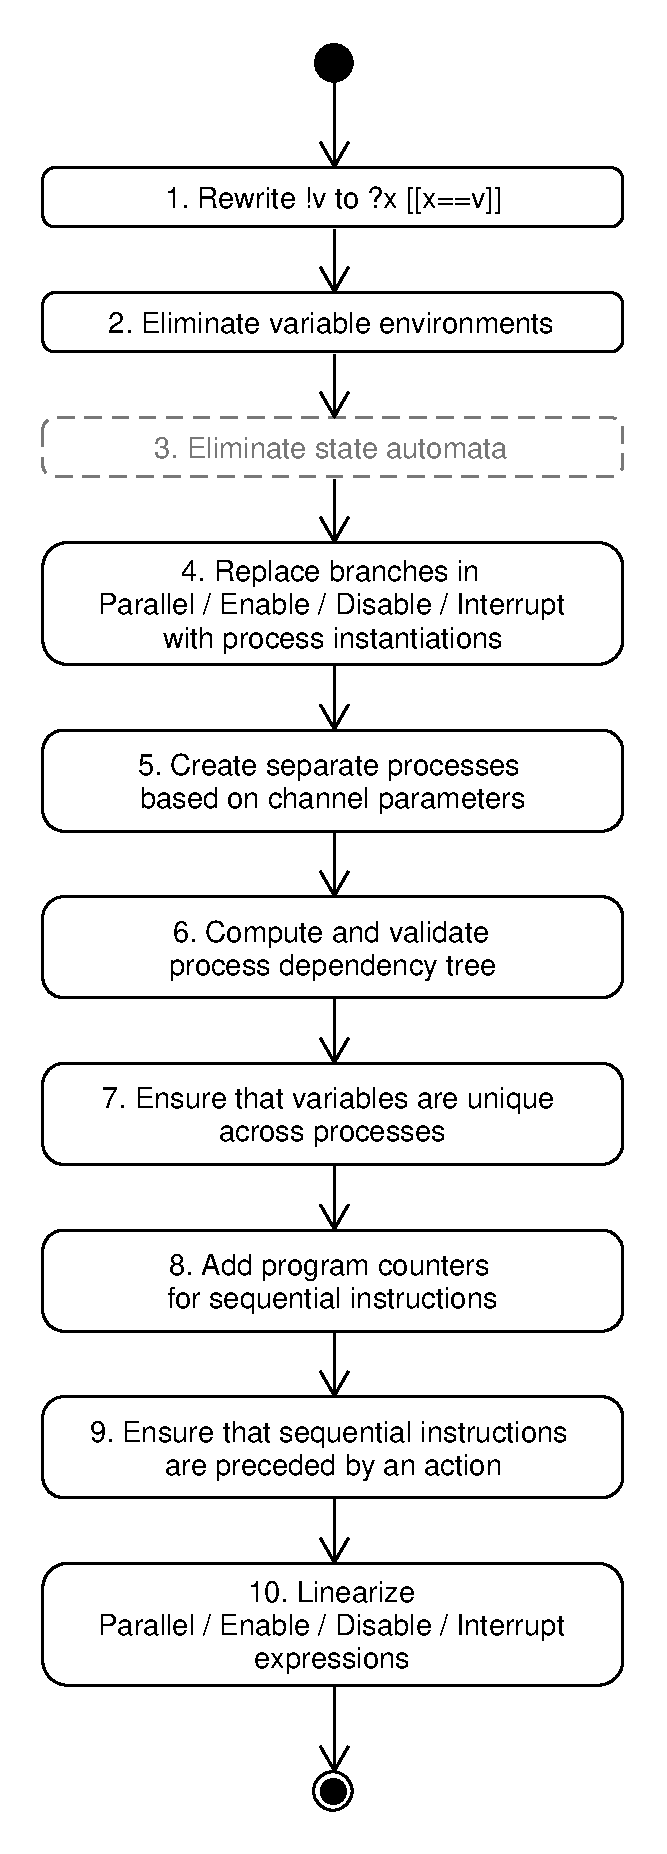
\includegraphics[width=0.5\linewidth]{umlet/linearization-main-flow}
\caption{Main flow.}
%\label{lpedatastructure:fig}
\end{center}
\end{figure}

\begin{figure}[!ht]
\begin{center}
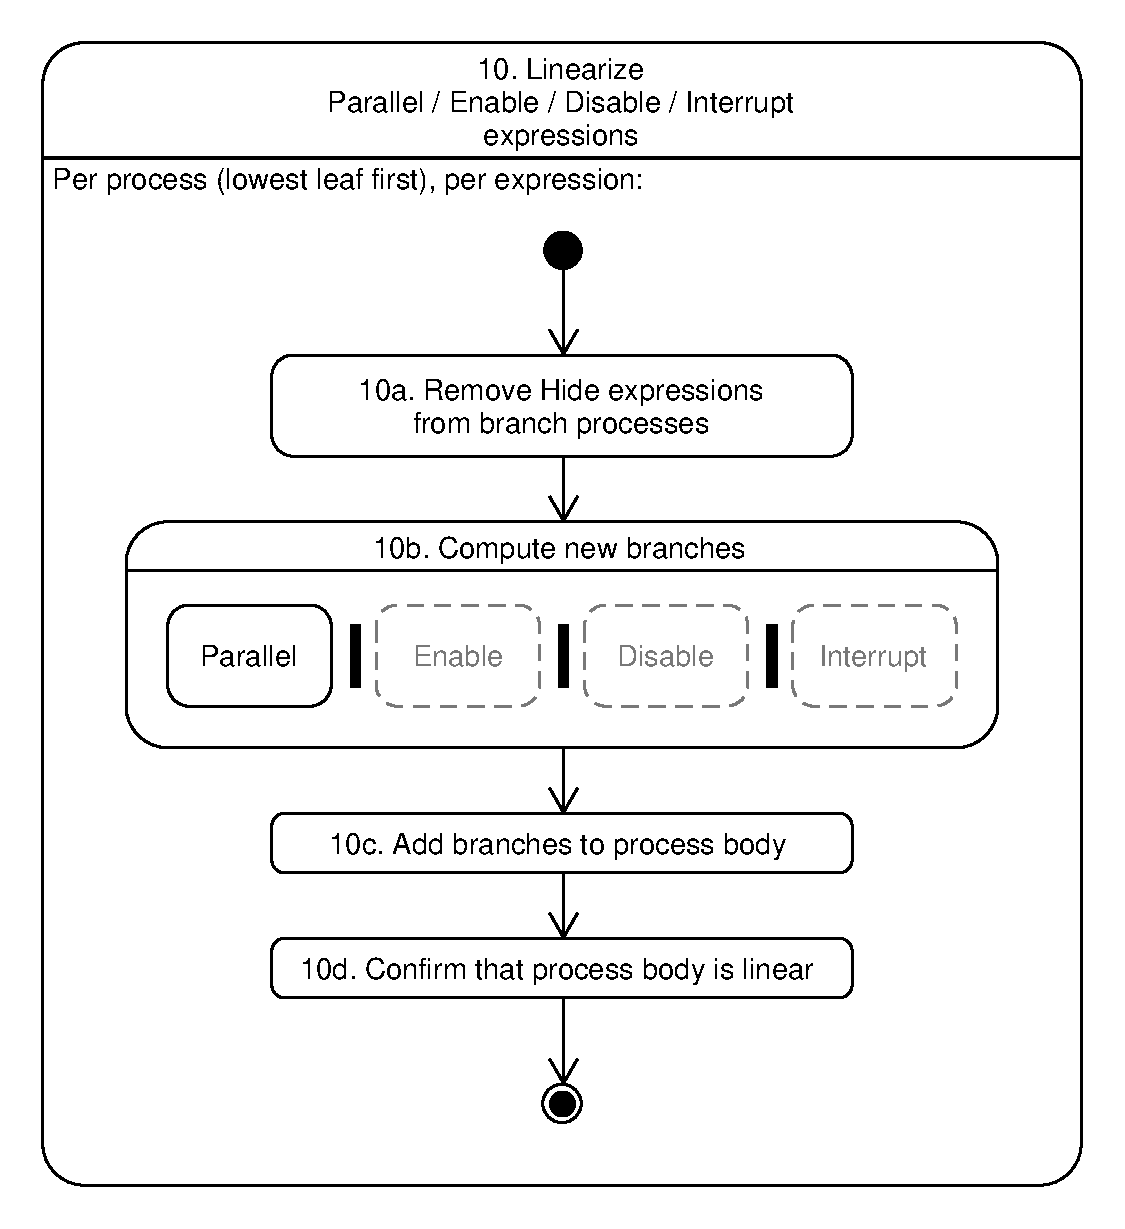
\includegraphics[width=0.8\linewidth]{umlet/linearization-pbranch-flow}
\caption{Main flow.}
%\label{lpedatastructure:fig}
\end{center}
\end{figure}

\bibliographystyle{plainnat}
\bibliography{biblio}

\end{document}
